% Compile from this directory: xelatex -interaction=nonstopmode TokenTrail_Project_Outline.tex
\documentclass[10pt,a4paper]{article}
\usepackage[margin=14mm,top=14mm,bottom=14mm]{geometry}
\usepackage{fontspec,graphicx,tabularx,booktabs,array,enumitem,hyperref,tikz}
\usepackage[table]{xcolor}
\usetikzlibrary{positioning,arrows.meta}
% Font fallback, so the file builds on macOS and Windows alike without
% requiring Microsoft Word to be installed: Helvetica Neue ships with macOS,
% Arial with Windows. On anything else the LaTeX default font is kept, which
% is always present. Arial is a little wider than Helvetica Neue, so a Windows
% build can run a line or two longer; both were checked to fit the same page
% count. The body is English; if Chinese text is added, load xeCJK as well.
\IfFontExistsTF{Helvetica Neue}
  {\setmainfont{Helvetica Neue}\setsansfont{Helvetica Neue}}
  {\IfFontExistsTF{Arial}
     {\setmainfont{Arial}\setsansfont{Arial}}
     {}}
\definecolor{navy}{HTML}{315E75}
\definecolor{teal}{HTML}{2E766E}
\definecolor{amber}{HTML}{A17431}
\definecolor{lightblue}{HTML}{EAF3F7}
\definecolor{lightteal}{HTML}{EDF6F2}
\definecolor{lightamber}{HTML}{FAF3E5}
\definecolor{lightrow}{HTML}{F7FAFB}
\definecolor{hairline}{HTML}{BDD0D8}
\arrayrulecolor{navy}
\hypersetup{colorlinks=true,urlcolor=black,linkcolor=black,pdftitle={TokenTrail Project Outline}}
\setlength{\parindent}{0pt}
\setlength{\parskip}{3pt}
\setlist[itemize]{leftmargin=15pt,itemsep=1pt,topsep=2pt}
\renewcommand{\arraystretch}{1.1}
\newcolumntype{Y}{>{\raggedright\arraybackslash}X}
\newcommand{\sect}[1]{\vspace{3pt}{\large\bfseries#1}\par\vspace{1pt}}
% Same as \sect, but forbids a page break immediately before or after the
% heading, so a heading and the unbreakable table under it stay together.
\newcommand{\sectkeep}[1]{\vspace{3pt}{\large\bfseries#1}\par\nobreak\vspace{1pt}}
\newcommand{\smallhead}[1]{{\bfseries#1}}
\newcommand{\tagline}[1]{\colorbox{lightblue}{\parbox{\dimexpr\linewidth-2\fboxsep}{#1}}}
\pagestyle{plain}
\begin{document}
\color{black}

{\fontsize{22}{26}\selectfont\bfseries TokenTrail}\hfill{\normalsize Android App Project Outline}\par
\vspace{3pt}{\color{navy}\hrule height 0.7pt}\vspace{4pt}
\textbf{Category:} Developer Productivity / API Cost Analytics\hfill\textbf{Target users:} API-key agent users.

\sect{1. App idea and user problem}
TokenTrail is an Android app for API-cost analytics, aimed at students and independent developers who use API-key coding agents: \textbf{Codex with OpenAI}, \textbf{ZCode with general Z.ai API access} and a DeepSeek-side tool to be selected. Its centre of gravity is \textbf{usage statistics}: the app opens on an \textbf{analytics home screen} that prices and compares the logged API usage behind those tokens. Two supporting parts sit behind it -- a \textbf{monthly tower-defence game} whose building resources come from the tokens the user has already spent, and a \textbf{community forum} carrying official model and pricing news. An \textbf{advice agent} sits on that home screen: it reads the user's usage records and recent forum posts, then answers questions with evidence. TokenTrail \textbf{does not run, route or control} the coding agents.

Scope is \textbf{API usage priced at public API rates}; ChatGPT and GLM Coding Plan subscriptions are excluded. A response reports tokens for one call, not the agent's history, and an API key cannot recover another agent's past per-call usage, so a call is priced only when a saved rate snapshot covers its date. Every monetary value is an \emph{estimate}, never an invoiced charge.

\sect{2. Related products and opportunity}
The review compares first-party API billing views with existing cross-model monitoring tools on data scope, cost provenance and decision support.\par
\begin{tabularx}{\linewidth}{@{}>{\raggedright\arraybackslash}p{27mm}Y Y@{}}
\toprule
\rowcolor{lightblue}
\textbf{Product} & \textbf{Relevant capability} & \textbf{Gap addressed by TokenTrail} \\
\midrule
\href{https://learn.chatgpt.com/docs/auth}{Codex} & Can run with an OpenAI API key, billed through the Platform account. & TokenTrail estimates only logged Codex API calls using dated OpenAI prices. \\
\rowcolor{lightrow}
\href{https://zcode.z.ai/en/docs/configuration}{ZCode} & Can use the general Z.ai API endpoint with an API key, separate from Coding Plan. & TokenTrail prices logged general-API calls, excluding plan usage. \\
\href{https://github.com/bowenliang123/dsh-context/blob/main/README.md}{dsh-context} & DeepSeek Harness plugin showing local sessions, token use, cache, activity and estimated costs. & TokenTrail spans API providers; session detail appears only when usable logs are imported. \\
\rowcolor{lightrow}
\href{https://docs.litellm.ai/docs/simple_proxy}{LiteLLM} & Open-source gateway with routing, spend tracking and budgets for proxied calls. & TokenTrail does not proxy traffic; it tracks agent-associated API costs from permitted records. \\
\href{https://github.com/zhu1090093659/dsh-pet/blob/main/README.zh.md}{dsh-pet} & Interactive floating pet driven by DSH session events, with touch and feeding actions. & TokenTrail adds cross-provider, evidence-linked advice, and turns consumption into a visible monthly progression. \\
\bottomrule
\end{tabularx}
\sect{3. Proposed contribution}
\textbf{Unified view.} TokenTrail merges authorised API-call logs from Codex, ZCode and a DeepSeek-side tool, removes duplicate records and shows source and coverage; session detail appears only where logs support it. \textbf{Reproducible costs.} Java applies dated official rates by provider, model, token class and service tier, and keeps the price version behind each estimate. \textbf{Reflected progress.} Tokens already spent on real work convert into building resources in a monthly tower-defence game, so a day of agent work leaves a visible result without asking the user to spend differently. \textbf{Decision support.} Activity and budgets help users understand spending and compare agents on computed measures only: logged token counts, dated rates, cache behaviour and duration. The app never asks the user to rate a task or judge an answer, so the analysis costs no extra input. An advice agent on the analytics home screen is the conversational interface, its read-only tools supply calculated evidence, and the model states sample size and missing data. It neither controls coding agents nor interrupts the workflow. Values remain \emph{Estimated}, \emph{Partial estimate} or \emph{Unavailable}.

\tagline{\textbf{Scope rule:} The three core parts are the API-cost analytics home screen, the monthly tower-defence game and the community forum; statistics are the app's main purpose, and the game and forum support it. The advice agent can recommend but cannot execute coding agents or enforce a hard cap. Subscription quotas, live cross-agent status and system-wide overlays are outside the first release.}

\sectkeep{4. Planned functionality and the four data aspects}
\begin{tabularx}{\linewidth}{@{}>{\raggedright\arraybackslash}p{27mm}Y Y@{}}
\toprule
\rowcolor{lightblue}
\textbf{Aspect} & \textbf{Planned implementation} & \textbf{User value / evidence} \\
\midrule
Data input & Coding-agent profile, key label and budget; authorised usage logs; user questions to the advice agent; forum posts. & Codex, ZCode and a DeepSeek-side tool; explicit source and coverage labels. \\
\rowcolor{lightrow}
Data processing & Java prices dated usage, compares agents by cost and converts spent tokens into game resources; the agent requests read-only summaries and drafts advice. & Advice cites data and exposes missing fields; no invented live activity. \\
Data storage & Firebase Authentication; UID-restricted Firestore; Room for usage, price versions, game state and advice history. & Historic estimates retain the price version used at calculation time. \\
\rowcolor{lightrow}
Data output & A home screen of Java/XML cost cards, a heatmap, sessions, budget alerts and the advice agent, backed by the game and the community forum. & A mobile view of spending and work patterns, with unavailable states for missing logs. \\
\bottomrule
\end{tabularx}

\sect{5. Core features and implementation approach}
The app opens on the \textbf{analytics dashboard} built from the first four bullets -- cost summary, sessions, comparison and budget -- and the advice agent is entered from there. The game and the forum are one tap away in the bottom bar.
\begin{itemize}
  \item \smallhead{Account and agent profiles.} Registration, login, logout and password reset. Users add Codex, ZCode and a DeepSeek-side tool as tracked profiles with a non-secret key label. No agent password is requested and no task is dispatched.
  \item \smallhead{API usage and cost.} Import user-authorised per-call usage logs; no agent must route traffic through TokenTrail. Record call time, model, agent, provider and input, cached-input and output tokens where available, de-duplicate calls and apply the matching saved price version. CNY display uses a dated exchange-rate snapshot.
  \item \smallhead{Session insights and efficiency.} When logs permit, group calls by session and show title, time, turns, tokens, cache hit, tool calls and duration; session cost is the sum of eligible call estimates. With only aggregate tokens, show provider-level estimates without inventing sessions.
  \item \smallhead{Budget and action.} Compare estimated spend with a user budget, showing coverage and uncertainty; forecasts use comparable history only. Alerts are advisory, not a cap on external agents, and no payment is handled.
  \item \smallhead{Monthly tower-defence game.} A supporting tab, not the landing screen: a tower-defence game played in monthly seasons that match the billing cycle AI subscriptions follow. Tokens already spent convert into building resources at a fixed rate per million tokens; resources buy and upgrade defences, walls and a data-centre base that expands in one direction. A wave starts only when the user begins one and runs in real time, so no offline simulation or scheduled settlement is needed. A season resets each month.
  \item \smallhead{Advice agent on the home screen.} The agent is entered from the analytics dashboard, where the figures it reasons about are already on screen; it opens an expandable question panel and reads two sources: the user's logged usage and recent forum posts. A Java service calls one selected external GPT, GLM or DeepSeek model, which may request \emph{getUsageSummary}, \emph{getBudgetStatus}, \emph{compareAgentCosts} and \emph{getForumHighlights} through function calling; Java executes and validates these read-only tools. Replies state evidence and missing data, no logs means no cost-based answer, and the agent's own tokens are tracked separately from coding-agent usage. It compares agents on cost and token use, never on output quality.
  \item \smallhead{API price updates.} Store official-rate snapshots with source URL, currency, model, token class, service tier and observation time. New rates apply prospectively and old estimates keep their version; where no contemporaneous rate exists, a current-price comparison is labelled uncertain rather than backdated.
\end{itemize}

\sect{6. Data flow and limitations}
\begin{center}
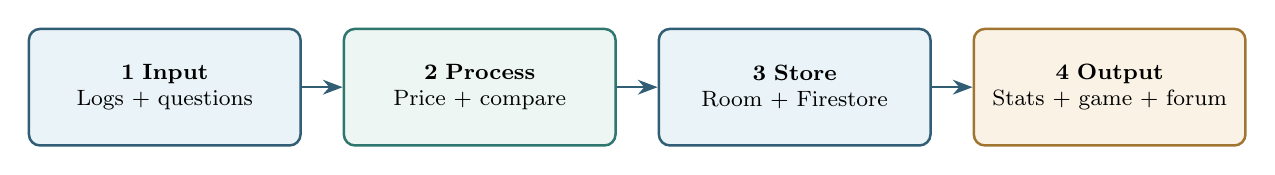
\begin{tikzpicture}[font=\footnotesize,flow/.style={rounded corners=4pt,minimum width=3.45cm,minimum height=1.48cm,text width=3.05cm,align=center,line width=.9pt,inner sep=4pt}]
\node[flow,draw=navy,fill=lightblue] (input) at (1.725,0) {\textbf{1  Input}\\Logs + questions};
\node[flow,draw=teal,fill=lightteal] (process) at (5.725,0) {\textbf{2  Process}\\Price + compare};
\node[flow,draw=navy,fill=lightblue] (storage) at (9.725,0) {\textbf{3  Store}\\Room + Firestore};
\node[flow,draw=amber,fill=lightamber] (action) at (13.725,0) {\textbf{4  Output}\\Stats + game + forum};
\foreach \a/\b in {input/process,process/storage,storage/action}{\draw[-{Stealth[length=2.5mm]},line width=.9pt,draw=navy] (\a.east) -- (\b.west);}
\end{tikzpicture}
\end{center}
Model responses report usage only for calls observed by the caller, so imported Agent logs are the primary input. Java matches token classes to dated prices, computes budgets and converts spent tokens into game resources; the external model receives selected summaries rather than API secrets or prompt text. A server-side function-call loop lets the agent query read-only tools, then return a short recommendation with source and coverage. The agent cannot observe a live coding session without a separate event feed.

\sect{7. Proposed Android interface}
The app opens directly into the \textbf{dashboard}: the analytics home screen holding Activity, Sessions, Compare and Budget, with the advice agent entered from it. Statistics lead because they are what the app is for -- what the API usage the user has already paid for actually cost. A bottom bar reaches the \textbf{game} and the \textbf{forum}. Inspired by dsh-context and dsh-pet, these sketches show summary metrics, a heatmap and forum cards. Log-dependent sections show an empty state when records are unavailable.
\vspace{2pt}
\begin{center}
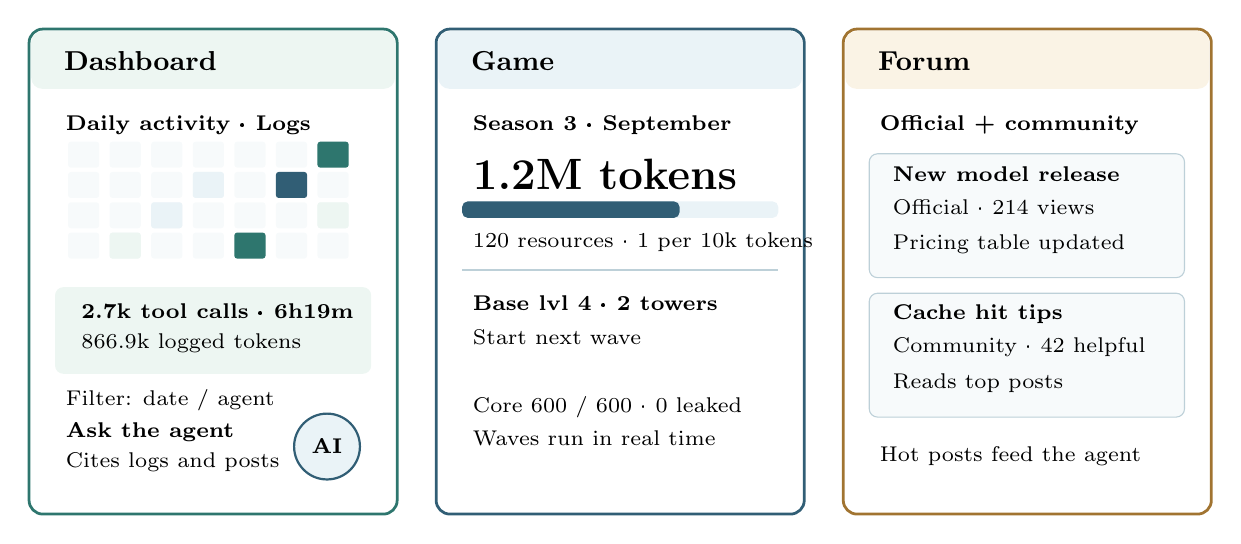
\begin{tikzpicture}[scale=1.1,transform shape,font=\scriptsize,every node/.style={text=black}]
% Three clean screen concepts; the home screen is drawn first. Colour is limited to borders, fills and data marks.
\foreach \x/\title/\border/\filltone in {0/Dashboard/teal/lightteal,4.7/Game/navy/lightblue,9.4/Forum/amber/lightamber}{
  \draw[draw=\border,line width=1pt,rounded corners=5pt] (\x,0) rectangle (\x+4.25,5.6);
  \fill[\filltone,rounded corners=4pt] (\x+.025,4.91) rectangle (\x+4.225,5.575);
  \node[anchor=west,font=\small\bfseries] at (\x+.28,5.23) {\title};
}
% Dashboard (the landing screen): daily heatmap from dated call or session records, and the agent entry.
\node[anchor=west,font=\scriptsize\bfseries] at (.3,4.49) {Daily activity · Logs};
\foreach \col in {0,...,6}{\foreach \row in {0,...,3}{\fill[lightrow,rounded corners=1pt] ({.45+0.48*\col},{2.95+0.35*\row}) rectangle ({.81+0.48*\col},{3.25+0.35*\row});}}
\foreach \col/\row/\tone in {1/0/lightteal,2/1/lightblue,4/0/teal,5/2/navy,6/1/lightteal,6/3/teal,3/2/lightblue}{\fill[\tone,rounded corners=1pt] ({.45+0.48*\col},{2.95+0.35*\row}) rectangle ({.81+0.48*\col},{3.25+0.35*\row});}
\fill[lightteal,rounded corners=3pt] (.3,1.62) rectangle (3.95,2.62);
\node[anchor=west,font=\scriptsize\bfseries] at (.48,2.34) {2.7k tool calls · 6h19m};
\node[anchor=west] at (.48,1.97) {866.9k logged tokens};
\node[anchor=west] at (.3,1.32) {Filter: date / agent};
\node[anchor=west,font=\scriptsize\bfseries] at (.3,.95) {Ask the agent};
\node[anchor=west] at (.3,.60) {Cites logs and posts};
\fill[lightblue] (3.44,.78) circle (.38);
\draw[draw=navy,line width=.8pt] (3.44,.78) circle (.38);
\node[font=\scriptsize\bfseries] at (3.44,.78) {AI};
% Game: monthly season, resources earned from tokens already spent. Reached from the bottom bar.
\node[anchor=west,font=\scriptsize\bfseries] at (5.0,4.49) {Season 3 · September};
\node[anchor=west,font=\Large\bfseries] at (5.0,3.92) {1.2M tokens};
\fill[lightblue,rounded corners=2pt] (5.0,3.42) rectangle (8.65,3.61);
\fill[navy,rounded corners=2pt] (5.0,3.42) rectangle (7.51,3.61);
\node[anchor=west] at (5.0,3.14) {120 resources · 1 per 10k tokens};
\draw[hairline,line width=.5pt] (5.0,2.82) -- (8.65,2.82);
\node[anchor=west,font=\scriptsize\bfseries] at (5.0,2.44) {Base lvl 4 · 2 towers};
\node[anchor=west] at (5.0,2.04) {Start next wave};
\node[anchor=west] at (5.0,1.24) {Core 600 / 600 · 0 leaked};
\node[anchor=west] at (5.0,.88) {Waves run in real time};
% Forum: official announcements plus community posts the agent can read.
\node[anchor=west,font=\scriptsize\bfseries] at (9.7,4.49) {Official + community};
\draw[draw=hairline,fill=lightrow,rounded corners=3pt] (9.7,2.73) rectangle (13.34,4.16);
\node[anchor=west,font=\scriptsize\bfseries] at (9.85,3.92) {New model release};
\node[anchor=west] at (9.85,3.54) {Official · 214 views};
\node[anchor=west] at (9.85,3.12) {Pricing table updated};
\draw[draw=hairline,fill=lightrow,rounded corners=3pt] (9.7,1.12) rectangle (13.34,2.55);
\node[anchor=west,font=\scriptsize\bfseries] at (9.85,2.31) {Cache hit tips};
\node[anchor=west] at (9.85,1.93) {Community · 42 helpful};
\node[anchor=west] at (9.85,1.51) {Reads top posts};
\node[anchor=west] at (9.7,.67) {Hot posts feed the agent};
\end{tikzpicture}
\end{center}
\vspace{-2pt}
\smallhead{Interaction and accessibility.} Each screen shows loading, empty and error states. Figures carry Agent, provider, estimate status, usage coverage, price version and refresh time; the heatmap has a numeric summary. A context ring is not API spend. The team checks touch targets, text scaling and screen rotation.

\sect{8. Technology and responsible reuse}
\begin{tabularx}{\linewidth}{@{}>{\raggedright\arraybackslash}p{33mm}Y@{}}
\toprule
\rowcolor{lightblue}
\textbf{Layer} & \textbf{Planned tools and rationale} \\
\midrule
Android interface & Java/XML, Material Components and Navigation; ViewModel/LiveData for state; RecyclerView and MPAndroidChart for trends; a tower-defence game surface and the advice agent panel on the home screen. \\
\rowcolor{lightrow}
Network and work & Retrofit/OkHttp for log import and a Java advice service. The service runs one model API and a bounded function-call loop over read-only usage, budget and comparison tools. WorkManager schedules price checks. \\
Persistence and security & Room plus UID-restricted Firestore; the Java service verifies Firebase ID tokens and holds its model key server-side. Imported metadata is protected; coding-agent passwords and keys are not required. \\
\rowcolor{lightrow}
Open-source reuse & Room with a View guides storage; MPAndroidChart may supply charts; an open-source tower-defence sample may supply the wave and placement loop; dsh-pet inspires the agent's entry point. Original or properly licensed art will be used, and reused files and licences recorded. \\
\bottomrule
\end{tabularx}

\sect{9. Work plan through the final submission}
The three-person team will follow the approximate course checkpoints: Alpha (weeks 8--9), Beta (weeks 11--12) and Final (weeks 15--16). The team will commit to GitHub throughout the project and adjust scope based on tested progress.\par
\begin{tabularx}{\linewidth}{@{}>{\raggedright\arraybackslash}p{24mm}Y >{\raggedright\arraybackslash}p{49mm}@{}}
\toprule
\rowcolor{lightblue}
\textbf{Course weeks} & \textbf{Work} & \textbf{Checkpoint / acceptance} \\
\midrule
1--3 & Confirm API-key agent use cases and UI; set up Firebase Auth and Firestore rules; document usage-log access and pricing dimensions. & Neither test account sees the other's records; token-source limits documented. \\
\rowcolor{lightrow}
4--7 & Implement agent profiles, usage-log import, Room/Firestore records, versioned pricing, CNY display and the analytics home screen. & Each provider's sample calls are priced at the correct dated rate and de-duplicated. \\
8--9: Alpha & Deliver a working login $\rightarrow$ add agent $\rightarrow$ import log $\rightarrow$ estimated cost $\rightarrow$ analytics path; separate real logs from sample data. & Source, description, GitHub link and MP4 per submission guidance. \\
\rowcolor{lightrow}
10--12: Beta & Add budgets and sessions; build the tower-defence loop (season, token-to-resource conversion, user-started waves); add the agent panel to the home screen and connect one model to three read-only tools. & The agent answers a usage question with evidence and admits missing data; a wave starts and resolves without blocking the UI. \\
13--15: Final & Evaluate advice accuracy and API cost, balance the season, improve accessibility, verify account isolation and document estimation limits. & End-to-end demo, report and video; no agent answer invents usage or controls coding agents. \\
\bottomrule
\end{tabularx}

\sect{10. Team work and evidence of completion}
Split by the three core parts. \textbf{Zhang Li (24107757)}: the data side -- authentication, usage-log import, Room/Firestore, versioned pricing, budgets and the dashboard. \textbf{Wang Tingdong (24107759)}: the forum, including its post data and ranking. \textbf{Liu Zongrun (24107745)}: the tower-defence game, the server-side agent service, its read-only tools and advice evaluation. UI/UX design, accessibility and integration are shared across all three, who each commit to GitHub. The interface between the game and the dashboard's figures is agreed jointly.

The demo opens on the statistics home screen and shows account isolation; tracked Codex, ZCode and DeepSeek-side profiles; three provider estimates from dated token logs; a heatmap and budget warning; then an agent question asked from that screen, such as ``Why did cost rise?'', answered with a queried summary, evidence and its own estimated API cost; finally a season in which those tokens became build resources.

Validation tests token accounting, price-version boundaries, missing usage, de-duplication and read-only tool limits, with the Firebase Emulator verifying access. Agent replies are checked against tool data, and the game is checked for a resource balance unreachable without logged usage. Published rates can differ from paid amounts; all figures remain estimates.

\sect{11. Functional requirements and improvements}
Each capability is mapped to what comparable tools already offer, what TokenTrail changes, and what is new. The advice agent runs on the analytics home screen, so its answers sit beside the figures they cite.\par
{\footnotesize
\begin{tabularx}{\linewidth}{@{}>{\raggedleft\arraybackslash}p{5mm}>{\raggedright\arraybackslash}p{32mm}Y>{\raggedright\arraybackslash}p{19mm}@{}}
\toprule
\rowcolor{lightblue}
\textbf{Ser} & \textbf{Existing features} & \textbf{Proposed improvements / new features} & \textbf{Remarks} \\
\midrule
1 & Cross-model cost dashboards & Three providers priced from dated official rates, de-duplicated, each figure carrying source and coverage & Improvement \\
\rowcolor{lightrow}
2 & Chat-history viewers & Per-call and per-session token-class breakdown, cache read and write split & Improvement \\
3 & Desktop context dashboards & Android client with Firebase Auth and UID-scoped rules & Improvement \\
\rowcolor{lightrow}
4 & Provider billing consoles & One cross-provider monthly budget with threshold alerts and a per-session breakdown & Improvement \\
5 & Community forums & Official model and pricing posts plus user tips, ranked for the advice agent & Improvement \\
\rowcolor{lightrow}
6 & Interactive pet with feeding (dsh-pet) & Monthly tower-defence season in which tokens already spent convert into build resources, with one-direction base growth and a wave the user starts & New feature \\
7 & General chat assistants & Advice agent on the home screen with function calling over read-only tools, reading usage records and hot forum posts & New feature \\
\bottomrule
\end{tabularx}}

\sect{12. Sources and project references}
\begin{tabularx}{\linewidth}{@{}>{\raggedright\arraybackslash}p{25mm}Y@{}}
\textbf{API scope} & \href{https://developers.openai.com/api/docs/pricing}{OpenAI pricing}; \href{https://api-docs.deepseek.com/quick_start/pricing/}{DeepSeek pricing}; \href{https://docs.z.ai/guides/overview/pricing}{Z.ai pricing}; \href{https://learn.chatgpt.com/docs/auth}{Codex billing modes}; \href{https://zcode.z.ai/en/docs/configuration}{ZCode endpoints}.\\
\textbf{Agent} & \href{https://developers.openai.com/api/docs/guides/function-calling}{Function calling}; \href{https://developers.openai.com/api/docs/libraries}{Java API client}; \href{https://firebase.google.com/docs/auth/admin/verify-id-tokens}{Firebase ID-token verification}.\\
\textbf{Related} & \href{https://github.com/bowenliang123/dsh-context/blob/main/README.md}{dsh-context dashboard}; \href{https://github.com/zhu1090093659/dsh-pet/blob/main/README.zh.md}{dsh-pet}; \href{https://docs.litellm.ai/docs/simple_proxy}{LiteLLM}; \href{https://github.com/android/codelab-android-room-with-a-view}{Room with a View}; \href{https://github.com/PhilJay/MPAndroidChart}{MPAndroidChart}.\\
\textbf{Security} & \href{https://firebase.google.com/docs/firestore/security/rules-conditions}{Firestore Security Rules conditions}.\\
\end{tabularx}

\end{document}
